\documentclass[12pt]{article}
% \usepackage{fullpage}
\usepackage{epic}
\usepackage{eepic}
\usepackage{paralist}
\usepackage{graphicx}
\usepackage{algorithm,algorithmic}
\usepackage{tikz}
\usepackage{xcolor,colortbl}
\usepackage{wrapfig}
\usepackage{float}
\usepackage{hyperref}


%%%%%%%%%%%%%%%%%%%%%%%%%%%%%%%%%%%%%%%%%%%%%%%%%%%%%%%%%%%%%%%%
% This is FULLPAGE.STY by H.Partl, Version 2 as of 15 Dec 1988.
% Document Style Option to fill the paper just like Plain TeX.

\typeout{Style Option FULLPAGE Version 2 as of 15 Dec 1988}

\topmargin 0pt
\advance \topmargin by -\headheight
\advance \topmargin by -\headsep

\textheight 8.9in

\oddsidemargin 0pt
\evensidemargin \oddsidemargin
\marginparwidth 0.5in

\textwidth 6.5in
%%%%%%%%%%%%%%%%%%%%%%%%%%%%%%%%%%%%%%%%%%%%%%%%%%%%%%%%%%%%%%%%

\pagestyle{empty}
\setlength{\oddsidemargin}{0in}
\setlength{\topmargin}{-0.8in}
\setlength{\textwidth}{6.8in}
\setlength{\textheight}{9.5in}


\def\ind{\hspace*{0.3in}}
\def\gap{0.1in}
\def\bigap{0.25in}
\newcommand{\Xomit}[1]{}

\author{Jonathan Gao}

\begin{document}

\begin{titlepage}
   \begin{center}
       \vspace*{5cm}
       {\huge\textbf{Slang}}
       \vspace{1.5cm}
       
       \textbf{Jonathan Gao}
       \vfill
       \vspace{0.8cm}
       Cornell University\\
       \today
            
   \end{center}
\end{titlepage}

\section*{Project Introduction}

\ind Slang is a friend discovery platform that allows friends to meet new people. The main feature of this app is the use of a queue system similar to those found in competitive multiplayer games, where players can queue with friends and teammates as a team. Slang aims to build on this idea, allowing groups of friends to queue together to find other groups of friends to meet. Along with some event suggestions, the app focuses around an effective matching algorithm. 

Rather than focus on individual to individual matching, Slang changes the game by building a group-based matching service. On Slang, groups of friends can queue together and search for new friends together, or even meet with other groups.

\section*{Project Scope}

\ind For this semester, I will be primarily focused on building the back-end infrastructure through AWS. This app will be built using AWS Amplify with a React Native front-end. 

For this prototype, I will be experimenting between two models of back-end infrastructure. With cloud computing, the standard model is to run computation through a virtual machine in the cloud. Typically, this means an EC2 instance from AWS that hosts a web server. In most cloud service providers, this virtual machine is elastic and will scale dynamically to the load of the web server. 

However, an alternative to the standard web server model is a server-less infrastructure. A server-less infrastructure uses simple functions as the back-end. Instead, the processing happens like a state-less state machine, where functions get called to process state transitions. The states get stored on the database service, thus the function only performs state transitions. This yields a model where our virtual machine doesn't need to store persistent state and lends itself to a more flexible and elastic infrastructure. Many cloud services offer lambda functions, which are allocated dynamically per function call. Thus, the back-end API will be implemented through lambda functions, which fetch and modify data stored in the database.

I am planning to use a NoSQL database, DynamoDB, which stores data as a key-value store. As the data Slang stores is not real-time or necessarily consistent, DynamoDB is a good service as it is scalable and eventually consistent. Using a key-value store, it is possible to use a file directory structure to store our information. For example, a profile can be mapped to a key ``slang/prod/profile/\{profileID\}'' which can then be hashed to store in the key-value store.

Extending this idea, I plan to keep all state in this database. 
\begin{itemize}
    \item Group profiles: \texttt{slang/prod/group/}
    \item Matches: \texttt{slang/prod/matches/}
    \item Invites: \texttt{slang/prod/invites/}
    \item Archives: \texttt{slang/prod/archives/...}

\end{itemize}

There are more data types, but they may be dependent on implementation.

For the front end, I plan on having periodic refresh events which fetch data from the back-end. However, if real-time chat is to be implemented, I can also look into implementing live updates. 

However, because much of the app depends on state changes in the front-end, we can rely on hooks to call the back-end API. The back-end doesn't really need to do any work on its own, so the server-less model can prove really useful and flexible.

\section*{Considerations}

\ind There are some issues that I may have to consider. While profile details and such are sized relatively small, delivering media content may be cost much more bandwidth. Storing these files in the database can likely dramatically slow down the back-end service, so I may try to use a content delivery network (CDN) to host media. This way, I can simply store a pointer to some media in which the front-end will fetch separately.

\section*{Current work}

Currently, Slang is in its design stages. Below are some mockups of the intended Slang interface.

\begin{figure}[H]
    \centering
    \caption{"Figma mockup of Slang"}
    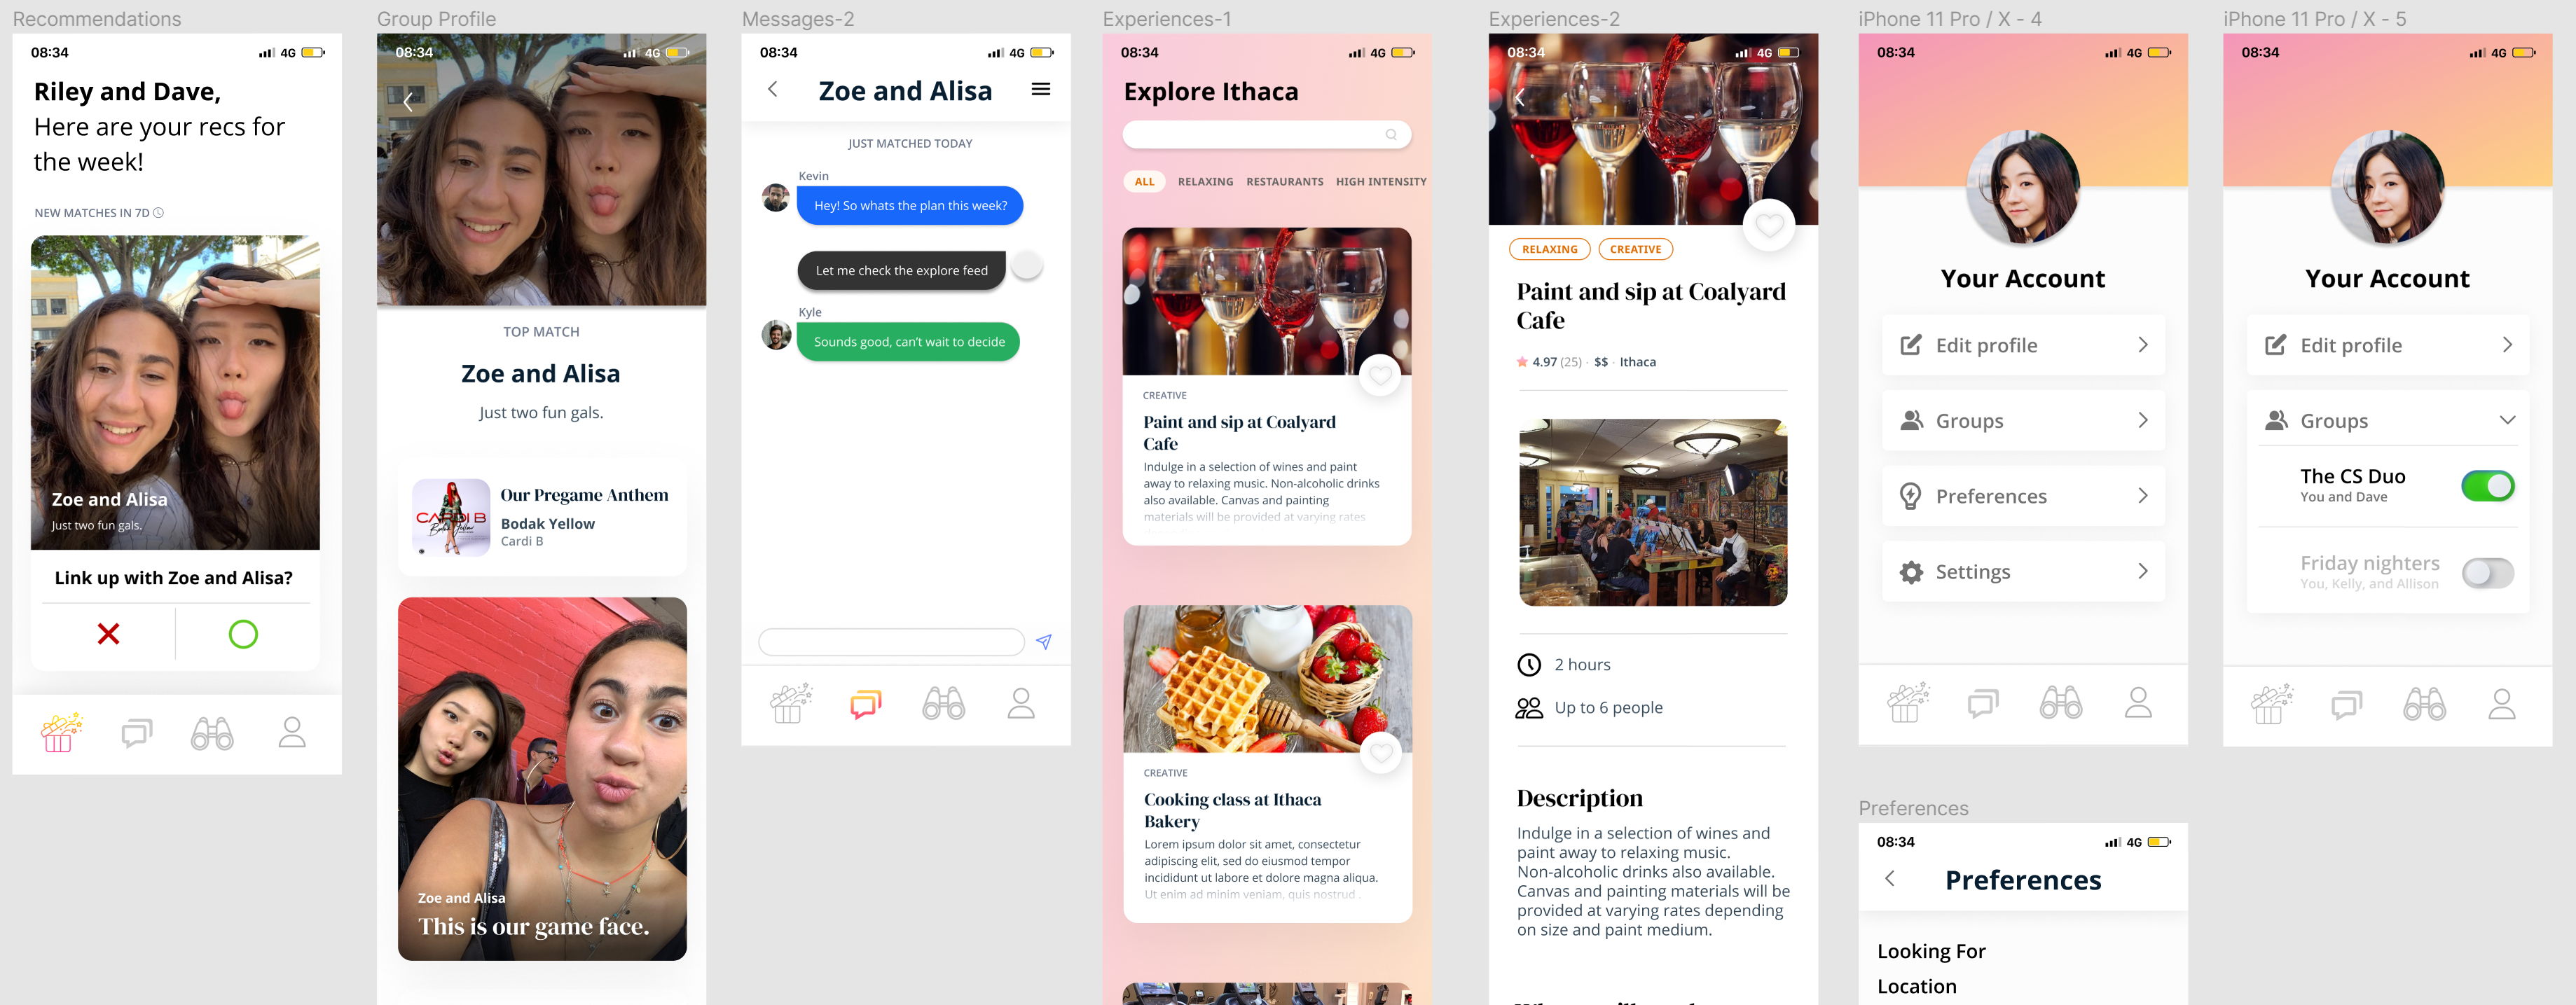
\includegraphics[width=\textwidth]{slang-figma.png}
\end{figure}

I have started working on a full-stack workflow on AWS, and the current deployed version can be found at \url{https://main.d3akp1i2vshy51.amplifyapp.com/one}
\end{document}

